\documentclass[11pt,letterpaper]{article}
\usepackage[T1]{fontenc}
\usepackage[utf8]{inputenc}
\usepackage{lmodern,amsmath,amssymb,amsthm,mathtools}
\usepackage[margin=1in]{geometry}
\usepackage{microtype,booktabs,tabularx,longtable,array,enumitem}
\usepackage{xcolor,graphicx,tikz,listings,fancyhdr}
\usepackage[hyphens]{url}
\usepackage{hyperref}
\definecolor{ink}{HTML}{18334A}
\definecolor{accent}{HTML}{007C83}
\definecolor{pale}{HTML}{F0F5F7}
\hypersetup{colorlinks=true,linkcolor=ink,citecolor=accent,urlcolor=accent,
 pdftitle={Cocycle Transport and Ordered Boundary Interfaces for Unknot Recognition},
 pdfauthor={ProveIt research continuation}}
\setlength{\headheight}{14pt}
\pagestyle{fancy}\fancyhf{}
\fancyhead[L]{\small\color{ink}Cocycle transport and boundary interfaces}
\fancyhead[R]{\small ProveIt / 9 October 2026}
\fancyfoot[C]{\thepage}
\renewcommand{\headrulewidth}{0.3pt}
\setlength{\parskip}{4pt}
\setlength{\parindent}{1.2em}
\setlist{itemsep=3pt,topsep=5pt}
\newtheorem{theorem}{Theorem}[section]
\newtheorem{lemma}[theorem]{Lemma}
\newtheorem{proposition}[theorem]{Proposition}
\newtheorem{corollary}[theorem]{Corollary}
\theoremstyle{definition}
\newtheorem{definition}[theorem]{Definition}
\newtheorem{example}[theorem]{Example}
\theoremstyle{remark}
\newtheorem{remark}[theorem]{Remark}
\newcommand{\Z}{\mathbb Z}
\newcommand{\N}{\mathbb N}
\newcommand{\R}{\mathbb R}
\newcommand{\pos}[1]{\left[#1\right]_{+}}
\newcommand{\rng}{\operatorname{rng}}
\newcommand{\bits}{\operatorname{bits}}
\newcommand{\poly}{\operatorname{poly}}
\newcommand{\code}[1]{\texttt{\detokenize{#1}}}
\newcommand{\baseline}{3a90fb34146c915328ab8eac6250cc2514f74ed0}
\lstset{basicstyle=\small\ttfamily,breaklines=true,columns=fullflexible,
 keepspaces=true,frame=single,rulecolor=\color{pale},backgroundcolor=\color{pale},
 showstringspaces=false,tabsize=4}

\begin{document}
\hypersetup{pageanchor=false}
\begin{titlepage}
\color{ink}
\noindent\textsc{Topology / Algorithmic research continuation}\par
\vspace{1.0cm}
{\huge\bfseries\noindent Cocycle Transport\\[0.12cm]
and Ordered Boundary Interfaces\par}
\vspace{0.25cm}
{\LARGE\noindent for Unknot Recognition\par}
\vspace{0.65cm}
{\large\noindent Exact Pachner scores, checked geometric descent,\par
\noindent and four-coordinate recovery of compressed attachment order\par}
\vspace{0.7cm}
\noindent Research continuation for the ProveIt project\par
\noindent 9 October 2026\par
\vspace{0.75cm}
\normalcolor
\begin{abstract}
We develop two concrete improvements to the geometric part of an unknot
recognition program. First, an integral simplicial cocycle is transported
through a checked $2$--$3$ or $3$--$2$ Pachner move using five integer
heights. We derive exact, constant-size formulas for the Euler-characteristic
change and the change in the number of normal discs of the coherent fibre.
They permit all eligible collapses to be scored in one incidence scan and
remove repeated cohomology elimination from a downward epoch. The edge
max-norm does not increase under $3$--$2$ moves and grows by at most a
factor of two under each $2$--$3$ move, giving an explicit bound on every
intermediate binary coordinate.

Second, we recover the cyclic order of finitely many marked occurrences on
a binary-encoded normal boundary curve. Removing the marks leaves paths
and unmarked circles. Because every path has exactly two endpoint
occurrences, its endpoint pair is recovered exactly from a count, a sum,
and a sum of squares. Together with path length, four additive coordinates
replace a vector whose dimension grows with the number of marks. This is
a deterministic encoding, with independently checked decoding and no
probabilistic fingerprints.

The implementation includes separate certificate consumers, source-bound
unknot witnesses, literal and Regina comparisons, adversarial tests, and
paired performance experiments. The local results advance retriangulation
and attachment handling. They do not bound the number of geometric escapes
needed for arbitrary diagrams, nor supply the complete three-dimensional
cutting compiler required by a general quasi-polynomial recognizer.
\end{abstract}
\vfill
\noindent\small\textbf{Audited repository revision}\par
\noindent\small\href{https://github.com/VladimirReshetnikov/ProveIt/commit/3a90fb34146c915328ab8eac6250cc2514f74ed0}{\texttt{3a90fb34146c915328ab8eac6250cc2514f74ed0}}\par
\noindent\small Main target: \path{Topology/UnknotRecognition/fast/}.\par
\noindent\small The supplied patch is additive; the existing recognition schedule remains unchanged.
\end{titlepage}

\hypersetup{pageanchor=true}
\pagenumbering{roman}
\tableofcontents
\clearpage
\pagenumbering{arabic}

\section{Results, scope, and the current baseline}

The useful next question is how to carry a compressed geometric object
through an actual change of triangulation, and how to retain the order
information needed to attach its boundary. An inventory of components is
insufficient for these tasks. Likewise, a fast certificate checker does not
give a bound for discovering a successful certificate. The present work
addresses two of these concrete interfaces and makes the remaining search
assumption explicit.

\subsection{What has been established}

The mathematical and implemented contributions are as follows.
\begin{enumerate}
\item An exact formula for the coherent-fibre Euler jump across a formal
bipyramid, valid for arbitrarily large integral heights and for the
generalized triangulations admitted by the checked move interface.
\item An exact nonnegative formula for the corresponding normal-disc
increase in the $2$--$3$ direction. Together, the formulas supply a
deterministic score for $3$--$2$ candidate discovery.
\item A cochain-preserving implementation of a complete downward epoch,
with independent replay of every move and an explicit coordinate-bit bound.
It solves cohomology once at entry, not once per accepted collapse.
\item A source-bound positive-certificate consumer. It checks the input
diagram's compact exterior, any preliminary boundary shellings, the
transported sequence, and a terminal essential-disc component certificate.
\item Exact recovery of marked boundary cycles, occurrence identities,
intervening lengths, and unmarked-cycle multiplicities. A four-coordinate
moment representation removes the increasing weight dimension from the
endpoint-identification query.
\end{enumerate}

The algebraic formulas and the two-endpoint decoding theorem are proved
below. The orbit engine, manifold validator, and normal-component kernels
are pre-existing project components. Their use is stated explicitly rather
than counted as newly implemented functionality.

\subsection{What the audited repository already contains}

The audit is pinned to \texttt{\baseline}; the live repository may continue
to change. At this revision, the main code already contains the direct
diagram-to-exterior construction and its independent replay, boundary
shellings, checked Pachner moves in both directions, primitive rank-one
cocycle extraction, minimum-span optimization, exact Euler optimization
on a certified minimum-span face, and compressed normal-component queries.
In particular, the diagram-to-exterior correspondence is no longer an
unimplemented entry step at this baseline \cite{ProveIt}.

The earlier coherent-escape study supplies an eight-tetrahedron solid-torus
example whose primitive coherent surface has genus two. It exhibits a
$3$--$2$ escape and investigates greedy simplification followed by fresh
cocycle extraction. The present contribution continues that experiment
with direct cochain transport and exact candidate scores. The old study
does not contain the five-height jump formulas or the moment endpoint
encoding derived here.

The incoming inventory was also checked. Ten relevant packages cover
quadrilateral-support kernels, sparse normal and port incidence, topology
spectra, compiled orbit certificates, weighted component certificates,
power-conjugacy methods, and selective orbit transfer. Their component
and profile interfaces are useful predecessors, but the inspected port
packages explicitly leave cyclic order and arbitrary pointwise attachment
maps outside their contracts. The present ordering interface addresses
finitely many distinct marked occurrences; it does not silently extend to
every pointwise gluing operation. The package contains a separate source
audit identifying these boundaries.

\subsection{Relation to primary literature}

Agol--Hass--Thurston supply the polynomial orbit and weighted-orbit
machinery for interval pairings \cite{AHT}. Lackenby's efficient-certification
paper uses such computations to recover ordered intersections around
vertical parallelity annuli; its proof of Theorem~9.2, especially
Section~9.4, is the theoretical predecessor of the marked-order interface
\cite{LackenbyCertification}. Our implementation specializes that established
method and reduces the number of additive coordinates by exploiting the
two-endpoint property.

Normal surfaces under Pachner moves, including the annulus-to-two-discs
configuration, are studied by Garoufalidis--Hodgson--Hoffman--Rubinstein
\cite[Section~12.4]{GHHR}. Their discussion makes an essential distinction:
an arbitrary normal surface may be transported with its topology preserved,
whereas transporting a cocycle and choosing its coherent fibre can change
the surface. Our exact score is for the latter operation. We claim a
derived formula and checked implementation in this project, not priority
for the underlying local surgery picture.

Polynomial-bit transport of cohomology during boundary simplification is
also established in Lackenby's Proposition~10.3
\cite{LackenbyCertification}. The elementary max-norm estimate below is
specialized to individual checked $2$--$3$ and $3$--$2$ moves.

Lackenby's 2021 slides state the announced running time
$2^{O((\log n)^3)}=n^{O((\log n)^2)}$ \cite{LackenbySlides}. His July 2026
preprint develops hierarchy algorithms and efficient certificates, including
the compressed cutting interface of Theorem~14.4, but does not state a
general quasi-polynomial runtime theorem \cite{Lackenby2026}. We therefore
use \emph{quasi-polynomial} in its usual broad sense
$\exp((\log n)^{O(1)})$, and state separately when a conditional result gives
the stronger $n^{O(\log n)}$ form.

\section{Integral cocycles and coherent normal fibres}
\label{sec:cochains}

\subsection{Encoding conventions}

Let $\mathcal T$ triangulate a compact three-manifold with $t$ tetrahedra.
Face pairings
are explicitly listed, while normal coordinates and cocycle values are
binary integers. Formal tetrahedron vertices may become identified in the
manifold. An oriented edge cocycle $z$ assigns an integer to every oriented
global edge, reverses sign under reversal, and has zero oriented sum around
every triangular face.

The native adapter further requires a connected orientable manifold with
exactly one torus boundary component. Closed, ideal, disconnected, and
other-boundary triangulations are outside this adapter's present contract.
The local identities below do not need all these additional restrictions.

On each tetrahedron choose four local heights
$h_0,h_1,h_2,h_3\in\Z$ such that
\[
 z(i\to j)=h_j-h_i.
\]
The face equations are exactly what permits these local lifts. On a paired
face the heights on one side differ from their transported counterparts by
a single integer constant. Thus the local affine functions define a
piecewise-linear map to $\R/\Z$. Its inverse image of
$\tfrac12+\Z$ is a properly embedded, cooriented normal surface, called
the \emph{coherent fibre} of $z$ in $\mathcal T$ and denoted $S(\mathcal T,z)$.
On every oriented edge its intersection signs agree.

Adding a constant to all four heights in a tetrahedron changes no local
normal coordinate. Our implementation normalizes the first local height to
zero. This convention controls representation size and makes independent
replay deterministic; it is not a vertex coboundary.

\begin{lemma}[Local normal coordinates]
\label{lem:local-coordinates}
Order the corners so that $h_a\le h_b\le h_c\le h_d$, resolving equalities
by the local vertex index. The coherent fibre contains
$h_b-h_a$ triangles at $a$, $h_d-h_c$ triangles at $d$, and
$h_c-h_b$ quadrilaterals separating $\{a,b\}$ from $\{c,d\}$.
Every other coordinate is zero. Its number of normal discs in that
tetrahedron is
\[
 P_t=\rng(h_0,h_1,h_2,h_3):=\max_i h_i-\min_i h_i.
\]
\end{lemma}
\begin{proof}
A half-integer level between the lowest and the second-lowest height cuts
off the lowest corner. A level between the middle heights separates two
corners from two, and a level between the second-highest and highest
height cuts off the highest corner. These three disjoint sets of levels
have the stated cardinalities. Tied heights create zero-length ranges and
require no exception. Their sum is the total height range.
\end{proof}

The construction handles exponentially many normal discs by a constant
number of integers per tetrahedron. It is nevertheless only one class of
normal surfaces. In particular, it suppresses pairs of oppositely signed
edge intersections; such a pair can occur in a topology-preserving normal
representative of the same cohomological data.

\subsection{Cohomology and a change of gauge}

For an integral vertex potential $p$, the cocycle $z+\delta p$ has local
heights $h_i+p(v_i)$. It represents the same cohomology class as $z$ but can
give a different coherent normal fibre. The existing project uses a
maximal-tree gauge to extract a primitive rank-one class, and can then
optimize the total number of discs over vertex potentials. Neither
primitivity alone nor an arbitrary change of gauge should be confused with
a proof that a subsequently transported fibre is connected.

Our positive consumer does not need a connectivity invariant throughout the
search. It checks a terminal normal vector with the existing component
kernel and requires that an essential disc occur as a component. This
permits the transported fibre to split or to contain additional components.

\subsection{The formal Pachner region}

Give a triangular bipyramid belt labels $C,D,E$ and apex labels $A,B$.
The two-tetrahedron filling is
\[
 \mathcal B_2=\{ACDE,BCDE\}.
\]
The three-tetrahedron filling is
\[
 \mathcal B_3=\{ABCD,ABDE,ABEC\}.
\]
The six boundary triangles agree. A $2$--$3$ move replaces
$\mathcal B_2$ by $\mathcal B_3$ and creates the interior edge $AB$;
the inverse $3$--$2$ move removes that edge.

A valid site must satisfy the full formal-region gluing conditions. Edge
degree three alone is insufficient. The native $3$--$2$ checker requires
three distinct tetrahedra, propagates the formal labels through their
interior faces, verifies the three expected vertex sets, and checks every
boundary face correspondence. Global boundary identifications of the formal
region are allowed by the existing checked contract. The interior cell
replacement is what matters for the argument below.

\section{Exact jumps across a bipyramid}
\label{sec:jumps}

\subsection{Five heights and preservation of the class}

\begin{lemma}[Local cochain transport]
\label{lem:transport}
An integral cocycle on either filling of a valid Pachner region determines
five heights $H_A,H_B,H_C,H_D,H_E$, up to an additive constant, by lifting
through the formal region. Restricting these heights to the other filling
defines a cocycle that agrees on every unchanged edge and represents the
same integral cohomology class under the move's relative-boundary
identification. Computing the five heights takes a constant number of
integer operations once the labelled region has been supplied.
\end{lemma}
\begin{proof}
Choose one local tetrahedron lift. On a shared interior face, all differences
of the three shared corner heights are prescribed by the cocycle, so the
lift on its neighbour is fixed by one additive adjustment. Propagation
through the two- or three-tetrahedron formal ball yields values on the five
labels. The cocycle condition makes different propagation routes consistent;
the implementation checks this consistency rather than assuming it.

The new edge values are differences of the same five values. They therefore
satisfy all new face equations and retain the values on the six boundary
triangles. On the formal ball both cochains are coboundaries of a local
height function. These functions agree at the boundary vertices, and their
affine extensions are homotopic relative to that boundary. Gluing this
local homotopy to the unchanged exterior shows that the two circle-valued
maps represent the same class. Equivalently, evaluate the cocycle on a
cycle and replace every segment crossing the ball by a boundary path;
both evaluations agree. The finite region has at most three tetrahedra,
so only a constant number of additions, subtractions, and comparisons occur.
\end{proof}

This lemma transports the cocycle. It makes no assertion that the fibres
before and after the move are isotopic.

\subsection{Closed formulas}

Sort the belt heights and the apex heights independently:
\[
 x\le y\le z\quad\text{are }H_C,H_D,H_E,
 \qquad L\le U\quad\text{are }H_A,H_B.
\]
Set
\begin{align}
 g&=\pos{L-z}+\pos{x-U},\label{eq:gap}\\
 \Delta P
 &=\max(U,y)-\min(L,y)
   +\pos{\min(U,x)-L}+\pos{U-\max(L,z)}.
 \label{eq:pieces}
\end{align}
Here $[r]_+=\max(0,r)$. The number $g$ is the gap between the closed
interval of belt heights and the closed interval of apex heights, taken
as zero when the intervals meet.

\begin{theorem}[Exact coherent-fibre jumps]
\label{thm:jump}
For cochain transport through a valid $2$--$3$ move,
\begin{align}
 \chi(S(\mathcal T_3,z_3))-\chi(S(\mathcal T_2,z_2))&=-2g,\label{eq:euler}\\
 P(\mathcal T_3,z_3)-P(\mathcal T_2,z_2)&=\Delta P\ge U-L\ge0.
 \label{eq:discjump}
\end{align}
The inverse $3$--$2$ move has Euler gain $2g$ and normal-disc saving
$\Delta P$. The statements concern the total coherent fibre, including all
its components. They remain valid with arbitrary integral heights, tied
heights, independent local additive offsets, and boundary identifications
allowed by the checked formal-region contract.
\end{theorem}

\begin{proof}[Proof by relative cell counts]
Write $r(a_1,\ldots,a_k)=\max_i a_i-\min_i a_i$.
Lemma~\ref{lem:local-coordinates} gives
\begin{align*}
 P_2&=r(L,x,y,z)+r(U,x,y,z),\\
 P_3&=r(L,U,x,y)+r(L,U,y,z)+r(L,U,z,x).
\end{align*}
Using $x\le y\le z$ and $L\le U$ and collecting the extrema yields
\begin{align}
 P_3-P_2={}&\max(U,y)-\min(L,y)\nonumber\\
 &+\min(U,x)-\min(L,x)
  +\max(U,z)-\max(L,z).\label{eq:pieces-alternate}
\end{align}
The difference of minima is
$[\min(U,x)-L]_+$, and the difference of maxima is
$[U-\max(L,z)]_+$. This proves~\eqref{eq:pieces}.
The first term is the range of $\{L,U,y\}$ and is at least $U-L$;
the other two terms are nonnegative.

For Euler characteristic, the unchanged boundary cell contributions cancel.
The old internal face $CDE$ contributes $r(x,y,z)=z-x$ normal arcs.
The new three internal faces contribute
\[
 r(L,U,x)+r(L,U,y)+r(L,U,z).
\]
The new internal edge $AB$ contributes $U-L$ intersection points.
There are no new interior vertices. Thus
\begin{align*}
 \Delta\chi={}&\Delta P
  -r(L,U,x)-r(L,U,y)-r(L,U,z)\\
  &+(z-x)+(U-L).
\end{align*}
Substitution of~\eqref{eq:pieces-alternate} cancels the terms containing
the median $y$ and gives
\[
 \Delta\chi=-|U-x|-|L-z|+(z-x)+(U-L).
\]
Use $|U-x|=(U-x)+2[x-U]_+$ and
$|L-z|=(z-L)+2[L-z]_+$ to obtain~\eqref{eq:euler}.

This proof is relative to the formal boundary, so identifications among its
cells do not change the cancellation argument. Only the replaced interior
faces and edge contribute to the difference. The reverse direction
negates both jumps.
\end{proof}

\subsection{An independent coarea check}

At a half-integer level, let $a\in\{0,1,2\}$ be the number of apices
above the level and $b\in\{0,1,2,3\}$ the number of belt vertices above it.
The following table gives $(\Delta\chi,\Delta P)$ for the two-to-three
replacement at that single level.

\begin{center}
\begin{tabular}{c@{\quad}cccc}
\toprule
 & $b=0$ & $b=1$ & $b=2$ & $b=3$\\
\midrule
$a=0$ & $(0,0)$ & $(0,0)$ & $(0,1)$ & $(-2,1)$\\
$a=1$ & $(0,2)$ & $(0,1)$ & $(0,1)$ & $(0,2)$\\
$a=2$ & $(-2,1)$ & $(0,1)$ & $(0,0)$ & $(0,0)$\\
\bottomrule
\end{tabular}
\end{center}

For example, when both apices are above all belt vertices, each old
tetrahedron contributes a triangular disc, while the three new quadrilaterals
form an annulus around the new edge. There are exactly $L-z$ such levels.
The reversed height ordering contributes $x-U$ levels. Summing gives the
gap formula. In other nonempty single-level cases the local surface is a
disc, although its subdivision and the number of pieces can change.

The table provides a second way to test the closed formulas and handles
ties without numerical limits. It is not an excuse to enumerate levels:
the implementation uses the five integers directly. In particular,
20,000-bit heights do not trigger $2^{20000}$ iterations.

Several exceptional annuli may be nested. We do not infer a family of
simultaneously disjoint compression discs for the entire original surface
from the single-level picture. The relative cellular proof already gives
the claimed global formula without this stronger geometric assertion.

\subsection{The existing obstruction as a numerical example}

In the repository's eight-tetrahedron example, one eligible collapse has
formal heights
\[
 (H_C,H_D,H_E,H_A,H_B)=(0,-1,1,3,4).
\]
Consequently $(x,y,z)=(-1,0,1)$ and $(L,U)=(3,4)$.
The gap is $g=2$, the Euler gain of the $3$--$2$ move is $4$, and
\[
 \Delta P=(4-0)+0+(4-3)=5.
\]
A checked downward epoch carries the original cochain through six
collapses, ending with two tetrahedra and an eight-piece normal disc.
The disc is established by the component certificate, not by substituting
the Euler gain into a connected-surface genus formula. The retained
record includes the preceding solid-torus construction; this particular
fixture is not presented as a witness for an independently supplied knot
diagram. Separate diagram-bound examples are tested below.

\subsection{Connectivity can fail: an explicit checked example}
\label{sec:splitting}

The archive includes a five-to-four-tetrahedron collapse whose incoming
primitive coherent fibre is one compressing disc with 24 normal pieces.
Its five heights, in belt-then-apex order, are
\[
 (0,2,1,5,4).
\]
Thus $(x,y,z)=(0,1,2)$ and $(L,U)=(4,5)$, giving $g=2$,
Euler gain $4$, and piece saving $5$. The outgoing fibre is one
11-piece compressing disc together with two four-piece spheres. Its
Euler characteristic is $1+2+2=5$ and its total piece count is $19$.
Both component censuses have independently replayed certificates.

The input arises from the existing interior-vertex solid-torus fixture,
an integral vertex coboundary, and one checked expansion. The coboundary
and transport preserve the primitive cohomology class. This provides a
direct counterexample to preservation of fibre connectivity under a legal
collapse, and to the proposed use of $\chi\le1$ for every transported
primitive fibre. It also explains why the source consumer uses the
general component kernel even when the initial seed was connected.

\begin{example}[Large geometric changes with short binary descriptions]
With $x=y=z=0$ and $L=U=H>0$, the upward move has
$\Delta\chi=-2H$ and $\Delta P=H$, although the new edge has cocycle
value zero. With $L=-H$, $U=H$, and the same belt, $g=0$ but
$\Delta P=4H$. These changes require only $O(\log H)$ input bits.
Neither unit Euler progress nor literal piece count is an appropriate
polynomial iteration budget; the formulas operate on encoded integers.
\end{example}

\section{Scored descent and binary complexity}
\label{sec:descent}

\subsection{One scan for all collapse scores}

The candidate scanner prepares the manifold once, groups its $6t$ local
edge occurrences by signed global edge class, and examines every degree-three
class. A class is accepted only when its three tetrahedra and interior
face maps form a valid labelled bipyramid. Each such test uses constant-size
local data. The five heights and the two scores are then obtained from
Theorem~\ref{thm:jump}.

The score policy chooses the largest Euler gain, then the largest disc
saving, with remaining ties resolved by local incidence order. A reference
policy chooses the first valid site. Every accepted move is constructed by
the existing Pachner producer and then checked independently. Every cocycle
transport is also checked independently using signed edge values and
global normal cell counts; the transport verifier does not call the score
formula.

\begin{proposition}[Candidate-discovery cost]
\label{prop:scoring}
After finite-manifold preparation, all eligible $3$--$2$ candidates and
their scores can be produced using $O(t)$ indexed operations and $O(t)$
integer operations on the input edge values. A score-based choice requires
one further linear scan. The candidate operation neither solves cohomology
nor expands a normal surface.
\end{proposition}
\begin{proof}
There are $6t$ local edge occurrences. Grouping visits each once. A rejected
group with a degree other than three is discarded by its recorded size;
each remaining group contains exactly three tetrahedra and at most twelve
face records. Label propagation, consistency checking, height lifting,
and score evaluation therefore take constant work per candidate.
There are at most $2t$ degree-three groups, which proves the bound.
\end{proof}

The statement counts indexed operations after the existing preparation
routine. Deterministic balanced dictionaries can replace expected-time
hash tables at an additional logarithmic factor. Python container costs,
certificate materialization, and the independent geometric checks appear in
the measured implementation time and are not hidden inside the constant-size
score claim.

\subsection{A complete downward epoch}

An epoch repeatedly discovers the eligible sites, chooses a site by the
fixed policy, performs the collapse, and transports the cochain. A move
limit can stop it early; the resulting transcript remains valid, but an
early stop is not declared a local minimum.

\begin{theorem}[Downward-epoch bounds]
\label{thm:epoch}
An uncapped $3$--$2$ epoch starting with $t_0$ tetrahedra contains fewer
than $t_0$ successful moves. Let
\[
 D_0=\max_e|z_0(e)|,\qquad
 B_0=\left\lceil\log_2(1+D_0)\right\rceil.
\]
At every stage the edge max-norm is at most $D_0$, each normalized local
height has absolute value at most $D_0$, and every normal coordinate is at
most $D_0$. The total normal-disc count never increases and the total Euler
characteristic never decreases. The entire epoch has polynomial encoded
cost in $t_0+B_0$, assuming the finite-manifold preparation and replay
operations used at a supplied state have their stated polynomial cost.
\end{theorem}
\begin{proof}
Every successful collapse removes one tetrahedron. A $3$--$2$ move removes
the edge $AB$ and creates no edge; every new tetrahedral edge is an old
boundary edge of the bipyramid. Lemma~\ref{lem:transport} preserves its
cocycle value. Hence the maximum absolute edge value does not increase.
After setting the first corner height to zero, the other heights are edge
differences from that corner. Each coordinate in
Lemma~\ref{lem:local-coordinates} is a difference along another tetrahedral
edge, so it has the same bound. The two monotonicity statements follow
from Theorem~\ref{thm:jump}.

There are $O(t_0)$ stages, each with $O(t_0)$ candidate work and a
constant number of supplied-state preparation, rewriting, and replay
operations. All arithmetic integers have $O(B_0+\log t_0)$ bits, including
the sums in global cell counts. Thus their composition is polynomial.
If all preparations are implemented by the native union--find and indexed
cell passes, the indexed work is $O(t_0^2\alpha(t_0))$ apart from dictionary
overheads and integer-bit costs. Retaining every full triangulation and
height array gives a quadratic-size transcript; the present code does retain
these arrays and claims no persistent-data-structure improvement.
\end{proof}

The theorem proves efficient completion of a geometric epoch. It does not
assert that the final coherent fibre contains a compressing disc. In
particular, Euler monotonicity is a statement about a sum over components,
not a connectedness theorem.

These complexity bounds use normalized initial height rows, or an edge-value
encoding of the cocycle. Arbitrary supplied additive offsets can have many
more bits than the edge differences. Their actual input length must be
included in the one-time reading and normalization cost. The identities
remain offset-invariant, and all subsequent transported rows satisfy the
advertised normalized-height bound. A quadratic-size transcript has
$O(t_0^2)$ integer slots, or
$O(t_0^2(B_0+\log(t_0+1)))$ bits including incidence indices.

\subsection{Upward moves and a precisely stated conditional search bound}

\begin{theorem}[Bit growth charged to upward moves]
\label{thm:upward}
Consider any sequence consisting of transported $2$--$3$ and $3$--$2$
moves, starting with $(t_0,z_0)$, and containing $u$ upward $2$--$3$ moves
in total. At every prefix,
\[
 t\le t_0+u,\qquad D\le 2^uD_0,
 \qquad B\le B_0+u.
\]
Accordingly, its current cocycle and normal-coordinate arrays use
$O((t_0+u)(B_0+u+1))$ bits, with an additional
$O((t_0+u)\log(t_0+u+1))$ bits for face-pairing indices.
\end{theorem}
\begin{proof}
Only an upward move can increase the number of tetrahedra. Its new edge
value satisfies
\[
 z'(A\to B)=z(A\to C)+z(C\to B)
\]
for any belt vertex $C$, so its absolute value is at most $2D$.
Every other edge value is retained. Downward moves do not increase $D$.
Induction gives the first two bounds. Since
$1+2^uD_0\le 2^u(1+D_0)$, the ceiling-logarithm bound follows. There are
four height and seven normal-coordinate entries per tetrahedron, and
Lemma~\ref{lem:local-coordinates} bounds each by the current $D$ after
normalization.
\end{proof}

This bound applies to the transported cochain. An algorithm that re-solves
cohomology and chooses a new vertex gauge introduces an additional operation
whose magnitude must be analysed separately. It also does not bound the
number of intermediate states visited by a search.

A path containing $u$ upward and $d$ downward moves has final size
$t_0+u-d\ge1$. Therefore $d\le t_0+u-1$, and its total number of moves
is at most $t_0+2u-1$. Storing a full state at every step uses
$O((t_0+u)^2)$ indexed records, each with
$O(B_0+u+\log(t_0+u+1))$ bits. This is a path-size bound. It does not
bound the number of possible paths, because many downward choices may
branch at each stage.

Fix a deterministic maximal downward policy $\mathcal D$. A
\emph{macrostate} is its output. A macrostep chooses one valid upward
move and then applies $\mathcal D$ again. Since a triangulation with $t$
tetrahedra has at most $2t$ paired faces, it has at most $2t$ candidate
upward sites of this kind.

\begin{corollary}[A bounded-escape macrofamily]
\label{cor:macro}
Exhaustively searching this specified macrofamily to upward depth $u$
visits at most
\[
 \sum_{j=0}^{u}\bigl(2(t_0+u)\bigr)^j
\]
macrostate tree nodes. Intermediate triangulations inside each deterministic
downward epoch are charged to that node's polynomial cost. With polynomial
complete supplied-state disc-component queries, the total cost is
\[
 \bigl(2(t_0+u)+1\bigr)^{u+1}
 \poly(t_0+u,B_0+u).
\]
For $t_0=\poly(n)$, $B_0=\poly(n)$, and $u=O(\log n)$ this is
$n^{O(\log n)}$. The completeness hypothesis needed for an input class
is that every unknotted input in that class has at least one macrostate in
this \emph{particular deterministic macrofamily}, within that depth, whose
coherent fibre contains an essential-disc component.
\end{corollary}
\begin{proof}
Theorem~\ref{thm:upward} bounds every encountered triangulation and integer
array. The number of children is at most $2(t_0+u)$ and each downward epoch
has polynomial cost by Theorem~\ref{thm:epoch}. Sum the breadth of the
depth-$u$ tree and apply the query bound.
\end{proof}

This is a mathematical reduction of the search target, not a completed
recognition theorem or an implemented exhaustive macrosearch. Different
downward choices can matter. Replacing all downward choices by one greedy
normal form without a coverage argument would be an invalid use of the
corollary. Nor does the existence of a short arbitrary Pachner path imply
the needed normal-form path bound. The shipped search implements a single
downward epoch; the corollary specifies a testable extension and its exact
remaining assumption.

\begin{remark}[Allowing bursts of upward moves]
The single-upward-move family is particularly restrictive: immediately
after an expansion its inverse collapse is valid, so the maximal downward
epoch performs at least one collapse. Macrostate tetrahedron counts can
never increase, and the global size peak is at most $t_0+1$ after the
initial closure. This family cannot represent an escape that requires
two consecutive expansions before any downward simplification.

A more flexible, still precisely bounded family lets each upward move
carry one additional decision: continue the current upward burst, or close
it by applying $\mathcal D$. Every nonempty accepted burst ends with a
close decision; the initial $\mathcal D$-state is also queried. At most
$u$ upward choices and $u$ binary closure choices occur on a branch.
There are at most $4(t_0+u)$ children per tree node, so
\[
 \sum_{j=0}^{u}\bigl(4(t_0+u)\bigr)^j
 \poly(t_0+u,B_0+u)
\]
bounds the work. This is again $n^{O(\log n)}$ for $u=O(\log n)$ and
polynomial initial size. No zero-length bursts are allowed. A witness
coverage theorem must now concern this larger, explicitly specified
family; it is still not a consequence of an arbitrary short Pachner path.
The burst variant is a research formulation, not shipped search code.
\end{remark}

\section{Ordered boundary data from compressed curves}
\label{sec:boundary}

\subsection{The information that component inventories lose}

Four marked occurrences $a,b,c,d$ can lie on the same circle in the cyclic
order $(a,b,c,d)$ or $(a,c,b,d)$. Their component-incidence vectors agree,
but gluing bands to those occurrences can produce different boundary
patterns. A hierarchy interface must therefore retain occurrence order,
not just the fact that the four marks are connected.

The following problem is intentionally narrower than constructing an
entire cut manifold. Its input is a degree-two graph already encoded by
interval pairings and a finite set of explicit marked vertices. Its output
is the first-return pairing between marked half-edges and the resulting
cyclic words. Actual normal boundary curves supply such inputs through the
existing native normal-arc compiler. A future three-dimensional parallelity
bundle compiler must supply analogous ordered interface curves and their
side labels.

\subsection{Multigraph and occurrence conventions}

\begin{definition}[Compressed boundary multigraph]
Let $V=[0,N)\cap\Z$. An affine interval pairing is a bijection
\[
 f:[a,b]\cap\Z\longrightarrow[c,d]\cap\Z,
\]
with slope $+1$ or $-1$ and $b-a=d-c$. For every domain point $q$,
the row contributes an undirected edge with endpoints $q,f(q)$. Distinct
rows or domain points define distinct edges, even when their endpoints
coincide. A loop counts twice toward degree. A compressed boundary graph
is a list of such rows whose multigraph has degree two at every vertex.
\end{definition}

Every connected finite degree-two multigraph is a circle, including a
one-vertex loop and a two-vertex circle with parallel edges. It is essential
to validate degree in this multigraph before passing to an orbit relation:
the orbit relation alone discards edge multiplicities and cannot validate
the hypothesis.

For $k$ pairing rows, degree validation is an endpoint-event sweep. Each
domain and range contributes $+1$ at its inclusive lower endpoint and $-1$
one past its upper endpoint. The running count must equal two on every
nonempty segment of $[0,N)$. This uses $O(k\log(k+1))$ comparisons of
binary endpoints and never visits all $N$ vertices.

Let $p$ distinct marked vertices, forming a set $M$, be supplied in an
explicit list. Their
positions in that list are occurrence identifiers; repeated display names
may be maintained by the caller, but duplicate geometric points are
rejected. A marked half-edge has the exact identity
\[
 (\hbox{pairing-row index},\ \hbox{original domain point},\
   \hbox{endpoint side }0\hbox{ or }1).
\]
This distinguishes both ends of a self-loop and parallel edges. There are
exactly $2p$ marked half-edges.

\subsection{Deleting marks without expanding the curve}

For each row, delete domain points that are marked, and preimages of
marked range points. Split the remaining domain into maximal integer
intervals. Then close the $p$ deleted gaps in the universe by the rank map
\[
 \rho(q)=q-\#\{m\in M:m<q\},\qquad q\notin M.
\]
On every surviving domain and range interval the rank map is a translation;
the induced pairing is therefore again affine with the original sign.

An original edge whose two endpoints are marked is recorded directly as
a zero-interior-length connection. Every other marked half-edge has one
unmarked neighbour; record that neighbour's compressed rank and the
half-edge label. The remaining graph has $N-p$ vertices. It consists of
paths with two missing endpoint incidences, and circles with no missing
incidence. An isolated unmarked vertex between two marks is a path of
length one in this convention and is included.

\begin{lemma}[Residual-size bound]
\label{lem:residual}
The residual graph has at most $k+2p$ interval-pairing rows. The number
of endpoint annotations is at most $2p$, independently of $N$.
\end{lemma}
\begin{proof}
The total number of edge occurrences incident to marks is at most $2p$,
because the marked degree sum is $2p$ and a marked-to-marked edge is
counted twice there. Removing $r_i$ distinct domain points from row $i$
leaves at most $r_i+1$ intervals. Hence the total is at most
$k+\sum_i r_i\le k+2p$. Each nondirect marked incidence produces exactly
one endpoint annotation.
\end{proof}

This sharper bound follows from degree two. The implementation uses binary
searches in the sorted mark list to find the relevant domain and range
marks; it does not need to scan every mark against every integer point.

\subsection{Four exact coordinates instead of one coordinate per port}

Assign the marked half-edges the distinct positive integer labels
$1,\ldots,2p$. For an unmarked vertex $v$, let $E(v)$ be the labels of the
missing incidences at $v$. Give $v$ the additive weight
\begin{equation}
 w(v)=\left(|E(v)|,\ \sum_{a\in E(v)}a,\
                \sum_{a\in E(v)}a^2,\ 1\right).
 \label{eq:moment-weights}
\end{equation}
The last coordinate is one on the entire residual universe. The other
coordinates are supported at at most $2p$ annotated vertices. Several
annotations at one vertex add exactly.

\begin{theorem}[Exact two-endpoint decoding]
\label{thm:moments}
Let $(c,s,q,\ell)$ be the orbit sum of~\eqref{eq:moment-weights} for a
component of the validated residual graph.
\begin{enumerate}
\item If $c=0$, then $s=q=0$ and the component is an unmarked circle
with $\ell$ vertices.
\item If $c=2$, the component is a path with two distinct marked
half-edge labels $a,b$. They are uniquely determined by
\[
 d^2=2q-s^2,
 \qquad a=\frac{s-d}{2},\quad b=\frac{s+d}{2},\quad a<b.
\]
The path has $\ell$ unmarked vertices. Its multiplicity in the orbit
histogram is one.
\end{enumerate}
There are no other cases. Thus four additive coordinates recover the same
endpoint matching and gap lengths as the $2p+1$-coordinate vector consisting
of an indicator for every port and one length coordinate.
\end{theorem}
\begin{proof}
Every residual component came from a circle after deleting some marked
vertices. If it meets no deleted incidence, it is a whole original circle.
Otherwise it is a path between two consecutive marked incidences, so it
has exactly two missing endpoint occurrences. These occurrences are
distinct half-edges, even when their marks are the same or the residual
path is a single vertex. Since labels are globally unique, their orbit
sum satisfies $c=2$, $s=a+b$, and $q=a^2+b^2$. Therefore
\[
 2q-s^2=2(a^2+b^2)-(a+b)^2=(a-b)^2.
\]
The nonnegative square root and the sum determine the unordered pair.
Two distinct path components cannot have the same pair of labels, since
each annotation occurs once, so a marked-path histogram record has
multiplicity one. The fourth coordinate counts its residual vertices.
Unmarked circles with the same length can and should be aggregated by
multiplicity.
\end{proof}

The decoder checks that $c$ is zero or two; in the second case it checks
that the discriminant is a positive exact square, that $s\pm d$ are even,
and that $1\le a<b\le2p$. It also checks that every port is used exactly
once after the direct connections are included. No floating-point square
root is used.

This argument depends on a proved two-endpoint bound. The first two moments
do not in general identify arbitrary multisets. For example,
$\{1,5,6\}$ and $\{2,3,7\}$ have the same size, sum, and sum of squares.
Consequently the four-coordinate decoder is not a general replacement for
all component-incidence vectors. Its exactness is supplied by the
validated boundary topology.

\begin{corollary}[Size of the moment query]
\label{cor:moment-size}
The query has dimension four, at most $k+2p$ pairing rows, and at most
$2p+1$ initially supplied weight intervals. Its nonlength coordinates have
$O(\log(p+1))$ bits under nonnegative weight transport, and its length
coordinate has $O(\log(N+1))$ bits. In particular, the moment encoding does
not hide a linear number of endpoint labels inside one exponentially long
integer.
\end{corollary}
\begin{proof}
Initially there are at most $2p$ endpoint annotations and one constant
length interval. The total first coordinate is at most $2p$, the total
label sum is at most $\sum_{a=1}^{2p}a=O(p^2)$, and the total square sum is
at most $\sum_{a=1}^{2p}a^2=O(p^3)$. All are nonnegative. Every stored
transported contribution is bounded by the respective conserved total.
The total length is $N-p$. These totals have the stated binary lengths.
The pairing bound is Lemma~\ref{lem:residual}.
\end{proof}

Combined with the weighted AHT theorem, this gives polynomial theoretical
time in the compressed input size and $p$. If overlapping supplied weight
intervals are converted into disjoint constant runs, the at most $2p$
annotated points give at most $4p+1$ runs, still $O(p)$; this is the
piecewise-constant weight-size parameter relevant to the orbit theorem.
The independently replayed
implementation is separately tested; the experiments do not constitute a
new formal proof of the orbit engine's running-time theorem.

\subsection{Recovering cyclic words and exact gaps}

The decoded connections define a fixed-point-free involution $\alpha$ on
the $2p$ marked half-edges, pairing the ends of every gap. At each mark,
the two incident half-edges define another fixed-point-free involution
$\tau$. Starting from an outgoing half-edge $h$, travel across a gap by
$\alpha$ and depart the next mark by $\tau$. Thus $\tau\alpha$ traces one
orientation of an original marked circle.

For each circle the default convention starts at its smallest occurrence
identifier and chooses the lexicographically smaller of the two directions.
A tie in a one- or two-mark circle is resolved by the outgoing half-edge
word, so the two sides of a loop remain distinguishable. The caller can
instead supply an explicit marked half-edge to fix the start and direction
on its own component.

Each output gap records the number $\ell$ of \emph{unmarked vertices}
between successive marks. It therefore contains $\ell+1$ original edges.
An entire marked cycle with $r$ occurrences contains
$r+\sum_i\ell_i$ vertices. The weighted replay preserves the residual
mass $N-p$, so reconstruction implies that marked cycle lengths plus
unmarked cycle lengths, counted with multiplicity, sum to $N$. Tests
also check this global equality explicitly.

The output includes exact half-edge descriptors, the gap matching,
canonical marked cycles, and a length--multiplicity histogram for circles
with no marks. It deliberately retains the latter: discarding a large
unmarked family would destroy the topology of a later cut representation.

\subsection{What remains outside this interface}

The marked graph does not by itself identify which side is horizontal in
an $I$-bundle, transport a meridian--longitude basis, or construct all
nonparallel pieces of a three-dimensional cut. A two-sheeted signed cover
is a natural way to extend the endpoint query to side parity, but that
extension is not claimed as shipped functionality here. Likewise, two
attachments at the same geometric point need a specified local ordering;
the current API rejects duplicate marked points.

Lackenby's compressed cutting theorem supplies the theoretical context for
these additional data. The present normal-boundary adapter exercises the
same ordered-curve primitive on actual normal arcs. It is a concrete
interface milestone, not the complete implementation of that theorem.

\section{Certificates and the source-bound positive search}
\label{sec:certificates}

\subsection{Separate mathematical responsibilities}

The implementation makes the following sequence checkable:
\begin{enumerate}
\item Reconstruct a valid classical one-component planar diagram and verify
its canonical compact exterior against the existing independent geometric
checker.
\item If preliminary boundary shellings were requested, verify the exact
removed tetrahedra and the resulting face pairings.
\item Validate the initial integral height rows and their signed global
edge consistency.
\item For every transcript step, verify the Pachner replacement, the
unchanged exterior, the five-height lift, the new height rows, the coherent
normal coordinates, and both global cell-count jumps.
\item Independently reconstruct the final coherent normal vector, replay
its compressed disc-component certificate, and require a strictly positive
number of essential disc components.
\end{enumerate}

Here an essential disc is a properly embedded disc whose boundary is
essential in the boundary torus. The final implication is the standard one:
the boundary of a knot exterior is compressible exactly for the unknot
\cite[discussion of Corollary 1.2]{Lackenby2026}.
Its use is justified here only after
the correspondence with the supplied diagram and every intervening
homeomorphism have been checked. A valid zero-disc certificate is rejected
as an unknot witness.

\subsection{The experimental positive stage}

\code{transport_seed_decide} constructs the canonical exterior, optionally
performs the existing boundary shellings, extracts one primitive integral
cocycle, optionally selects its existing minimum-span representative, and
performs one deterministic downward epoch. It submits the final vector to
the general compressed disc-component kernel. The return value is
\code{UNKNOT} with a complete certificate, or \code{INCONCLUSIVE}.
It never returns \code{KNOTTED} from failed coherent-fibre search.

The stage is an additive experimental API. It is not enabled in the
maintained recognition schedule. The move cap, shared work allowance, and
orbit-cycle allowance are explicit. The work allowance counts cooperative
guard invocations, not machine instructions or bit operations. All stages,
including positive certificate replay, share that allowance. Exceptions
raised by the caller's cancellation callback propagate.

\subsection{Independent replay and its limits}

The cocycle transport checker imports neither a transport producer nor a
cocycle solver. It does not call the score formula: it reconstructs signed
edge values and computes the old and new normal Euler characteristics from
the cell structure. The source consumer imports independent exterior,
shelling, move, and component checkers. Tests patch the discovery and
producer entry points to raise exceptions while the consumer continues to
verify a positive proof.

The marked-order checker independently reconstructs the degree-two source
graph, the deleted-mark instance, the endpoint weights, and the cyclic
solution, and then replays the supplied weighted orbit trace. Its certificate
is bound to the ordered pairing rows and the original mark list; relabelling
or reordering those inputs without changing the certificate is not accepted.

Shared low-level integer and finite-geometry routines remain part of the
trusted code base. These checkers are independent algorithmic replays,
not a Lean formalization or a separately verified implementation of every
supporting library. The archive records the exact code and test scope so
that this distinction is reviewable.

\section{Reproducible experiments}
\label{sec:experiments}
\newcommand{\ScoringLocalMax}{20.519}
\newcommand{\ScoringRestartMax}{6\,857.931}
\newcommand{\ScoringSpeedupMax}{334.23}
\newcommand{\BoundaryTraceMax}{4\,215}
\newcommand{\BoundaryReplaySpeedupMax}{14.16}
\newcommand{\BoundaryCombinedSpeedupMax}{10.31}
\newcommand{\BoundaryMomentBytes}{344\,445}
\newcommand{\BoundaryBasisBytes}{507\,862}

\newcommand{\FullTestCount}{1\,289}


\subsection{Environment, baselines, and units}

The experiments use CPython 3.12.14 on Linux x86-64. Independent native
comparisons use the Regina Python distribution 7.4.1, whose engine reports
version 7.4 \cite{Regina}. The archive contains the source inputs,
certificate-bearing records, benchmark drivers, and an environment record.
All times in the tables are wall-clock milliseconds on the research
machine; they are measurements of the stated workloads, not complexity
exponents fitted from a few points.

The all-candidate scoring comparison uses five trials per arm, alternating
which arm runs first. The final endpoint-encoding comparison uses three
alternating trials per arm on identical normal curves and mark lists.
Raw samples are retained for those paired comparisons. The literal curve
walk is capped at 200,000 represented vertices; omitted larger walks are
not timed or extrapolated. The initial exploratory records are retained
separately and are not substituted for the matched comparison.

The machine is shared. Controlled measurements were run with other heavy
research jobs paused, but hardware isolation and a distribution over
machines are not claimed. Median ratios are descriptive. They do not
include uncertainty estimates, and the complete recognizer may spend most
of its time in a different operation.

\subsection{Exact score checks and independent native moves}

The local audit evaluates all $5^5=3,125$ five-height assignments in
$\{-2,-1,0,1,2\}^5$. It compares the formulas with separate tetrahedron,
face, and edge range counts. The regression also scales heights by
$2^{20000}$ and confirms unchanged deterministic guard counts, while the
arithmetic integers themselves become longer. This checks the absence
of a loop over represented levels; it is not a claim that big-integer
arithmetic has constant cost.

A seeded mixed-move audit performs 120 moves: 63 upward and 57 downward.
The four starting inputs are layered solid tori with two and eight
tetrahedra, a one-crossing diagram exterior, and a trefoil exterior.
Each accepted move passes independent cocycle replay. Regina's separate
Pachner operation gives an isomorphic replacement triangulation, and its
normal-surface Euler characteristic agrees with the native cell count.
The observed edge-magnitude ratio attains two in an upward move, so the
factor-two bound cannot be uniformly improved for this max-norm.

The eight-tetrahedron obstruction and the connectivity counterexample
from Section~\ref{sec:splitting} are retained with complete construction
data and component certificates. The former finishes after six collapses
with two tetrahedra and one eight-piece compressing disc, saving 33 pieces
overall. The latter verifies the split into a disc and two spheres.
Neither fixture is mislabeled as a proof about an unrelated diagram.

\subsection{All eligible collapse scores: a matched comparison}

The benchmark begins with layered solid tori of sizes
$16,32,64,128,256$. Expanding disjoint pairs gives the sizes and eligible
collapse counts in Table~\ref{tab:scoring}. These triangulations have one
global vertex. Therefore two primitive cocycles for the rank-one group
differ only by overall sign: there are no nonzero vertex coboundaries.
The coherent normal vector is unchanged by that sign. This makes fresh
cohomology extraction and direct transport comparable on exactly the same
geometric outputs.

The reference arm first recognizes eligible sites without scoring them.
For every site it constructs the full replacement triangulation, extracts
a fresh primitive rank-one cocycle, and computes its Euler characteristic
and normal-disc count. The new arm obtains every score directly from the
input cochain in one scan. The driver requires equality of all per-site
Euler and piece outputs before collecting timings.

\begin{table}[htbp]
\centering
\small
\begin{tabular}{rrrrrr}
\toprule
$t$ & Sites & Bits & Local (ms) & Fresh $H^1$ (ms) & Ratio\\
\midrule
24 & 8 & 13 & 0.933 & 18.597 & 19.93$\times$\\
48 & 16 & 24 & 1.894 & 71.151 & 37.57$\times$\\
96 & 32 & 46 & 3.855 & 300.348 & 77.92$\times$\\
192 & 64 & 90 & 8.259 & 1\,300.017 & 157.40$\times$\\
384 & 128 & 179 & 20.519 & 6\,857.931 & 334.23$\times$\\
\bottomrule
\end{tabular}

\caption{Scoring all eligible collapses. Times include each arm's stated
preparation and discovery work. The speedup is the ratio of median times.
Height bits grow with the layered family.}
\label{tab:scoring}
\end{table}

At the largest measured input, direct scoring takes
\ScoringLocalMax{} ms versus \ScoringRestartMax{} ms for the fresh-extraction
arm, a \ScoringSpeedupMax{}-fold ratio. This is not a
\ScoringSpeedupMax{}-fold speedup of unknot recognition.

The comparison also has an asymptotic explanation independent of the
timings. There are $\Theta(t)$ candidate sites in this family. The reference
arm explicitly materializes a whole $\Theta(t)$-size triangulation for
each site, so those writes alone cost $\Omega(t^2)$ indexed operations.
The new scoring stage uses $O(t)$ integer operations after preparation.
Cohomology elimination, integer-bit costs, and final successful-certificate
construction are additional costs with their own bounds.

\subsection{Diagram corpus: unchanged coverage is a result}

The maintained source audit supplies 84 source cases. The experiment
selects the 82 with at most sixteen crossings, reconstructs each diagram's
canonical compact exterior, and compares three supplied-coherent-vector
strategies:
\begin{enumerate}
\item the first eligible collapse followed by a fresh tree-gauge cocycle;
\item the first eligible collapse with the original cochain transported;
\item the maximum Euler-gain, then maximum piece-saving collapse with
the original cochain transported.
\end{enumerate}
The shared descent-and-query allowance is two million cooperative guard
calls per arm, with a terminal orbit limit of 5,000 cycles. The initial
canonical exterior and seed construction precede this measured arm budget.
The separate source API charges its own full pipeline to a shared budget.

All 246 arm runs complete. Every arm performs 144 collapses in total and
finds 15 positive disc-component cases. All 30 positive transport runs
pass the independent diagram/exterior/transport/component consumer.
Thus this experiment shows no additional recognition coverage.

Final Euler characteristics agree across all three arms on all 82 sources.
The two transport policies also have identical final piece counts on every
source. Fresh gauge extraction changes that count on twelve sources:
its total is 16,170, compared with 16,297 in either transport arm.
Accordingly, these data do not establish that the score ordering produces
better final geometry than first-site transport on the ordinary diagram
corpus. They demonstrate correct reuse and identify a workload where the
proposed priority is neutral.

The corpus record contains timings for diagnosis, but they are not a
matched speed comparison. In particular, full source replay was included
for positive transport runs, and the exploratory collection briefly
overlapped another audit. The scoring table above is the controlled
performance evidence. Positive proofs are replayed again from the
packaged records; source cases whose coherent query fails remain
inconclusive rather than being classified as knotted.

\subsection{Marked-order correctness and endpoint-encoding performance}

The marked-order feature tests compare 500 seeded signed interval-exchange
multigraphs with a literal edge-occurrence oracle. One hundred further
cases compare both weight encodings on the same input. Tests include
one-vertex loops, reflection fixed points, parallel rows, adjacent marks,
singleton residual paths, empty and all-marked graphs, and directed
traversal starting at each port of an adversarial example.

The native tests use normal meridians in layered solid tori, boundary
caps, and compatible disc/sphere/M\"obius mixtures. Eighteen boundary counts
are independently compared with Regina. Source pairing order, occurrence
order, encoded integer fields, weights, claimed cycle orders, and trace
events are mutated in rejection tests. Work limits and delayed callback
exceptions are also exercised.

For the paired encoding comparison, the input is a 64-tetrahedron native
normal boundary with 89,891,140,425,706 represented vertices and four raw
interval pairings. Only the number of explicit marks changes. The moment
and one-hot arms receive the same ordered rows and marks and must return
the same solution.

\begin{table}[htbp]
\centering
\small
\begin{tabular}{rrrrrr}
\toprule
Marks & \multicolumn{2}{c}{Producer (ms)} & \multicolumn{2}{c}{Replay (ms)} & Replay\\
 & Moments & One-hot & Moments & One-hot & ratio\\
\midrule
8 & 6.482 & 7.693 & 9.987 & 15.086 & 1.51$\times$\\
32 & 32.110 & 51.145 & 72.514 & 260.093 & 3.59$\times$\\
128 & 462.465 & 710.939 & 1\,062.141 & 15\,035.489 & 14.16$\times$\\
\bottomrule
\end{tabular}

\caption{Matched endpoint encodings on one native boundary. Producer times
include certificate recording. Replay is measured separately with the
independent consumer. All times are milliseconds.}
\label{tab:encoding}
\end{table}

At 128 marks the weight dimension falls from 257 to four, while both
encodings use \BoundaryTraceMax{} AHT events. Independent replay improves
by a factor of \BoundaryReplaySpeedupMax{} in this experiment.
The serialized certificate sizes are \BoundaryMomentBytes{} bytes and
\BoundaryBasisBytes{} bytes, respectively. The retained orbit trace limits
the overall size reduction even after dense endpoint vectors are removed.

There is still substantial growth with the number of marks. The output
itself has $2p$ ports, deletion creates more interval pieces, and the orbit
trace can become longer. The four-coordinate theorem removes a growing
dimension; it does not remove all dependence on $p$ or establish a
uniform constant-factor advantage.

\begin{figure}[htbp]
\centering
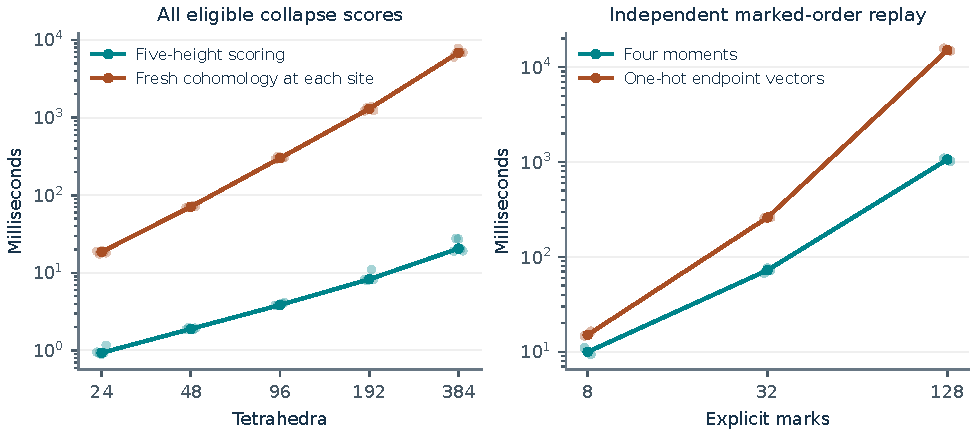
\includegraphics[width=\textwidth]{figures/paired_performance.pdf}
\caption{Paired measurements on logarithmic axes. Left: all-candidate
scoring; right: independent marked-order replay. Dots show individual
retained samples and lines join medians. No asymptotic slope is fitted.
Both comparisons require identical mathematical outputs.}
\label{fig:performance}
\end{figure}

\subsection{Literal controls and a 20,019-bit boundary size}

The retained native-boundary experiment with 22 tetrahedra, eight marks,
and 150,050 represented vertices takes 2.197 ms for the certified producer
and 3.121 ms for independent replay. The geometry-and-order wrapper takes
3.007 ms; this wrapper timing does not include the additional independent
replay. A literal native-arc walk takes 149.076 ms. Its ratio is
67.85 against the producer alone, or 28.03 against producer plus replay.
These particular medians were collected before the final callback-only
verifier correction; the interval algorithm and represented inputs are
unchanged. The final paired encoding table was regenerated after that
correction.

Small inputs favor literal walking. At 26 vertices the literal walk takes
0.046 ms versus 0.825 ms for the producer; at 1,220 vertices the times
are 1.058 ms and 1.495 ms. In 101 interleaved zero-mark controls on the
26-vertex case, moment replay takes 0.07024 ms versus 0.06827 ms for
one-hot replay, about 2.9\% slower. With one mark the corresponding
times are 0.09115 ms and 0.09023 ms. For zero or one mark the reference
dimension is one or three, so the four-coordinate representation should
not be expected to win universally.

A different input multiplies the 24-tetrahedron normal vector by
$2^{20000}$. The boundary size is
\[
 N=392836\cdot2^{20000},
\]
requiring 20,019 bits. Eight marks leave eight residual pairings from
four source rows. The recorded producer time is 8.614 ms, independent
replay 12.421 ms, and native-wrapper time 10.158 ms. The certificate
has 755,802 bytes and 108 AHT events. Three boundary components contain
marks; the remaining untouched family is retained with exact
multiplicities, giving $2^{20000}$ components overall.

This last experiment tests dependence on binary encoding and preservation
of multiplicity. It neither expands nor literally checks every represented
component, and it is not a benchmark of recognizing a knot with
$2^{20000}$ crossings.

\subsection{Regression and retained-proof validation}

The packaged snapshot passes \FullTestCount{} tests in the full
\code{unittest} discovery run, including the existing repository suite
and the new features. The retained-proof validation checks the
source-bound transport positives, the obstruction transcript, the
connectivity counterexample, and the correspondence between computed
table entries and their stored data. The machine-readable validation
record distinguishes full-suite tests, feature tests, proof replays, and
benchmark comparisons.

An initial full-suite attempt exposed a missing historical test oracle in
the standalone snapshot, not a mathematical failure. The exact pinned
\path{reports/24/reference/graded_transfer_v1.py} and the other required
historical oracle files are now included. The final full-suite run is
performed from the deliverable snapshot, with no references to an
unshipped checkout.

The validation supports this source revision and these contracts. It is
not a proof that all possible triangulations or all possible cancellation
schedules have been tested. Mathematical claims rest on the stated
proofs and hypotheses; implementation confidence additionally rests on
independent replay, adversarial examples, and the retained regression.


\section{Consequences for the quasi-polynomial program}
\label{sec:program}

The present results make two costs more explicit. A geometric collapse
epoch need not pay repeated global cohomology elimination, and a marked
attachment query need not carry one additive coordinate per marked
half-edge. Neither optimization supplies a bound on the number of
retriangulations or useful surface choices.

The most useful form of a future global theorem would control three
quantities simultaneously: the number of candidate continuations at a
state, the number of successive decisions or resets, and the bit size of
every state. Theorem~\ref{thm:upward} settles the third quantity for the
specific transported-cochain move sequence, once the number of upward
moves is bounded. Corollary~\ref{cor:macro} states the remaining coverage
assumption without suppressing the choice of downward policy.

There is also an unavoidable output-size issue for a literal full-cut
triangulation: arbitrarily many parallel normal components can leave
arbitrarily many intervening product components. A compressed cutter must
retain multiplicities, use an output-sensitive bound, or restrict its input
components. The unmarked-cycle histogram and binary normal coordinates in
this package are designed to preserve this information. Expanding them at
the next interface would discard the gain.

\subsection{A proved score refinement ready for implementation}
\label{sec:peeled}

The splitting example shows why raw Euler gain can reward the creation
of vertex-link spheres. The following exact refinement removes that
particular effect without restoring a global computation at every
candidate. It is a proved data-structure lemma; the refined scorer is
not implemented or benchmarked in this package.

For each global vertex $v$, let $C_v$ be its local tetrahedral corners
and let $a_c$ be the triangle coordinate at corner $c$. The maximal
vertex-link multiplicity is
\[
 m_v=\min_{c\in C_v}a_c.
\]
Writing $L_v$ for the vertex-link normal vector, define
$\operatorname{peel}(a)=a-\sum_v m_vL_v$. These subtractions preserve
nonnegativity, matching, and the quadrilateral condition. In normal
position the innermost complete triangle layers form the corresponding
disjoint vertex-link components. With
$\lambda_v=\chi(L_v)$, equal to one at a boundary vertex and two at an
interior vertex,
\[
 \chi(\operatorname{peel}(a))=\chi(a)-\sum_v\lambda_vm_v.
\]
This operation removes vertex links only; it does not include the
quadrilateral-gcd division in the existing full canonical-core routine.

\begin{proposition}[Thirteen corner records suffice]
\label{prop:peel}
During one scoring pass on a fixed triangulation and coherent vector,
retain at each global vertex its thirteen least triangle-coordinate
records, or all records if fewer exist. Break ties by corner identity.
After this $O(t)$-operation preparation, the exact vertex-link minima
after each legal $3$--$2$ candidate, and hence its peeled Euler jump, are
computable in $O(1)$ integer operations per candidate.
\end{proposition}
\begin{proof}
A candidate removes twelve old corners and supplies eight new corners.
If any old corner of an affected global vertex survives, its least
surviving record is among the first thirteen: otherwise at least thirteen
records would have been removed. Remove the deleted corner identities
from the retained list and compare the least survivor with the at most
eight new coordinates. If no old record survives, use infinity for that
temporary minimum; the legal replacement supplies a new corner for the
same global vertex.

There are at most five affected global vertex classes, even if some
formal vertices are identified. A constant-capacity heap constructs each
thirteen-record list in linear total work. The legal relative-boundary
move preserves the global vertices and their boundary/interior types,
so their link Euler characteristics are unchanged. All unaffected
triangle coordinates remain fixed under cochain transport. These facts
give both the claimed minima and the bound.
\end{proof}

In particular,
\begin{equation}
 \Delta\chi_{\mathrm{peeled}}
 =2g-\sum_{\text{affected }v}\lambda_v(m'_v-m_v).
 \label{eq:peeled}
\end{equation}
The counterexample has raw gain four and peeled gain zero, because its
two new vertex-link spheres account for the full difference. The peeled
piece count has the similarly exact change
\[
 \Delta P_{\mathrm{peeled}}
 =\Delta P_{\mathrm{raw}}
 -\sum_{\text{affected }v}(m'_v|C'_v|-m_v|C_v|),
\]
where $\Delta P_{\mathrm{raw}}=-\Delta P$ in the collapse direction.

\begin{corollary}[Peeled piece count is nonincreasing]
\label{cor:peeled-pieces}
Under coherent $3$--$2$ transport, the global vertex-link multiplicities
satisfy $m'_v\ge m_v$, and the number of normal pieces after vertex-link
peeling does not increase. This statement excludes global regauging and
quadrilateral-gcd division.
\end{corollary}
\begin{proof}
Put
\[
 a=[\min(U,x)-L]_+,\qquad b=[U-\max(L,z)]_+.
\]
These are the minimum old triangle coordinates at the lower and upper
formal apex. The new apical minima are $a+g$ and $b+g$.
At a belt vertex, its minimum over the local corners is unchanged.
Indeed, the triangle coordinate at height $h$ is its distance to the
interval spanned by the other three tetrahedral heights. The two old
intervals overlap on the apex interval; the two new intervals overlap
on the interval of the other belt vertices. Both unions are the interval
spanned by the other four heights. Taking the minimum distance gives
the same value.

Taking further minima over identified formal vertices and over unchanged
exterior corners proves $m'_v\ge m_v$. Let $r_v$ count the formal apices
identified with $v$. Then $|C'_v|=|C_v|-2r_v$ and
$\sum_v r_vm_v\le a+b$, also when the apices are identified. Projection
onto $[L,U]$ gives
\[
 a=\operatorname{clamp}_{[L,U]}(x)-L,\qquad
 b=U-\operatorname{clamp}_{[L,U]}(z).
\]
Since $x\le z$, we have
$a+b\le U-L\le\rng(L,U,y)$, and hence
$\Delta P=\rng(L,U,y)+a+b\ge2(a+b)$.
Writing $\delta_v=m'_v-m_v\ge0$, the peeled change is
\begin{align*}
 \Delta P_{\mathrm{peeled}}
 &=-\Delta P+2\sum_v r_vm_v-\sum_v\delta_v|C'_v|\\
 &\le-2(a+b)+2(a+b)=0.
\end{align*}
\end{proof}

This corollary is independently checked on all 3,125 small-height
assignments and all 52 partitions of the five formal vertices, with
additional exterior-minimum controls: 812,500 exact algebraic cases in
total. These tests do not assert that every partition is realized by a
legal ambient triangulation. The corollary does not establish monotonicity
of the peeled Euler characteristic, or a bound on the number of choices
needed to discover an essential disc.

These summaries must be rebuilt after committing a move or maintained by
a separately justified dynamic structure. Repeatedly deleting from a
thirteen-element list without replenishing it is invalid. The lemma also
requires that coordinates outside the candidate region remain unchanged;
it does not cover simultaneous global regauging. Whether the resulting
priority improves essential-disc discovery is a separate experimental
question, and non-vertex-link spheres still require component analysis.

\subsection{Proposed research questions and concrete milestones}

\begin{enumerate}[label=\textbf{Q\arabic*.},leftmargin=*]
\item \textbf{A bounded-escape coverage theorem.} Does a useful, explicitly
defined class of unknot diagrams have a successful coherent-fibre witness
in the deterministic macrofamily of Corollary~\ref{cor:macro}, or its
explicit upward-burst extension, at depth
$O(\log n)$? A first target should name the diagram class and the exact
downward policy. A counterexample should distinguish lack of a short
macro-path from mere failure of one bounded execution.

\item \textbf{Exchange of downward moves.} Under what conditions do two
eligible collapses commute, or admit a common descendant with the same
coherent boundary data? Proving a local exchange theorem could justify
collapsing many orders to one macrostate. Without such a theorem, retaining
one greedy order can lose coverage.

\item \textbf{Incremental geometric preparation.} Maintain signed edge
classes, degree-three candidate sites, and the five-height scores across a
move. The current implementation rebuilds prepared geometry. An update
algorithm must handle edge classes affected by global face identifications,
not only the visible formal vertices, and must have an independently
replayable update contract.

\item \textbf{Compact transcripts with local reconstruction.} The supplied
transcript stores whole intermediate triangulations and can occupy
quadratic space. Can an independent consumer reconstruct each next
triangulation from the local proof and a stable cell-name map, retaining
only a linear-size current state and a nearly linear transcript?

\item \textbf{Gauge optimization after transport.} Study reuse of the
minimum-span dual certificate and the Euler-optimal face after a local
move. A correct incremental method must account for the changed tetrahedral
objective and distinguish harmless local height normalization from a
global vertex coboundary. Compare both candidate coverage and full replay
cost with a fresh exact solve.

\item \textbf{Peeled scoring and connectivity through the exceptional slab.}
Implement Proposition~\ref{prop:peel} and compare the refined score with
raw Euler gain on source-bound examples. Give a precise
global description of the nested annulus-to-disc replacements, including
which components split and whether a selected essential-boundary component
can be followed without a fresh full census. The additive Euler formula
alone is insufficient for this purpose.

\item \textbf{A three-dimensional attachment compiler.} From a normal
surface and a triangulation, construct the nonparallel cut pieces and the
degree-two curve systems along each vertical parallelity component. Feed
their marked occurrences to the present ordering interface. The milestone
is one independently checked cut with ordered attaching squares and
horizontal-side correspondence.

\item \textbf{Signed endpoint transport.} Implement the two-sheeted cover
extension for side parity and compare it with direct signed path weights.
Specify what happens to an unmarked orientation-reversing circle and ensure
that the cover does not erase bundle multiplicity.

\item \textbf{Higher bounded endpoint valence.} For an interface whose
residual components have at most $d$ endpoints, can the first $d$ exact
power sums replace a unit-vector weight system with a practical decoder?
Newton identities give an algebraic route, but root recovery, multiplicity,
integer coefficient growth, and independent replay all need explicit bounds.
The two-endpoint case here is unusually simple and should remain the
baseline for performance comparisons.

\item \textbf{Certified input-sensitive scheduling.} Predict when moment
boundary queries or cochain descent will save actual time. The scheduler
must be evaluated on complete recognition and should charge failed
candidate searches. A local kernel speedup does not justify unconditional
activation on every diagram.

\item \textbf{An adversarial geometric corpus.} Build reproducible unknotted
families with growing upward escape requirements, and nontrivial knots
whose low-complexity coherent candidates are misleading. Retain all
negative results and resource-limited runs. Include true source diagrams,
not only triangulations with a known construction history.

\item \textbf{Formal verification of the small kernels.} The five-height
identities, endpoint-moment decoder, degree-two deletion lemma, and
source-consumer implication are suitable small formalization targets.
Their machine checking would reduce the trusted mathematical core while
leaving the larger AHT and three-manifold infrastructure as explicit
dependencies.
\end{enumerate}

\appendix
\section{Implementation and reproduction guide}
\subsection{Archive layout and integration}

The archive contains a complete source snapshot needed by the supplied
tests, an additive patch against the audited commit, the article sources
and rendered PDF, raw measurements, certificate-bearing audit records,
compact source cases, reproduction scripts, and provenance notes. The
\path{fast/} snapshot preserves the pinned files and adds the new modules.
Its sibling \path{reports/} directory contains only historical oracle
dependencies required by the existing tests.

The patch uses paths rooted at \path{Topology/UnknotRecognition/fast/}.
It adds the feature modules, tests, and research drivers. It does not alter
the production recognition schedule. The new article and the retained
data are separate reviewable artifacts; the repository's intake process
can place them under its next report number.

From a checkout at the pinned revision, inspect and check the patch:
\begin{lstlisting}
git apply --stat /path/to/integration.patch
git apply --check /path/to/integration.patch
\end{lstlisting}
The package build verifies that the patch applies to the pinned source
and reproduces its included added files. A later repository revision
should be checked independently for path conflicts before applying it.

\subsection{Python setup and tests}

The new native algorithms use the Python standard library. The maintained
project supports Python 3.10 or later. This research environment uses
Python 3.12.14; use Python 3.12 for the pinned optional package set.
Regina is optional for most native tests but required to
repeat the advertised independent Regina comparisons. The archive gives
the exact optional package versions in \path{requirements-research.txt};
it does not bundle third-party binary distributions.

A reproducible environment can be prepared at the extracted archive root:
\begin{lstlisting}
python3 -m venv .venv
. .venv/bin/activate
python -m pip install -r requirements-research.txt
python reproduce/run_checks.py --full
\end{lstlisting}
Without the optional dependencies, native feature checks can be run with:
\begin{lstlisting}
python reproduce/run_checks.py
\end{lstlisting}
The latter command uses standard-library test discovery and verifies
retained native proofs. Its output identifies optional comparisons
that were skipped. For the explicit repository regression:
\begin{lstlisting}
cd fast
python -m unittest discover -s tests -v
\end{lstlisting}

\subsection{Minimal source-bound example}

From the supplied \path{fast/} directory:
\begin{lstlisting}[language=Python]
from fastunknot import Diagram
from fastunknot.normal_transport import transport_seed_decide
from fastunknot.normal_transport_verify import (
    verify_transport_disk_certificate,
)

diagram = Diagram.from_braid(2, [1])
answer = transport_seed_decide(
    diagram, strategy="score", max_work=2_000_000
)
assert answer["status"] == "UNKNOT"
assert verify_transport_disk_certificate(
    diagram, answer["certificate"]
)
\end{lstlisting}

The function accepts optional boundary shellings and initial minimum-span
optimization. It performs no subsequent cohomology solve after a move.
A failed or resource-limited search returns \code{INCONCLUSIVE}. The
certificate schema is \code{diagram-transport-disc-v1}; it includes the
source PD, canonical exterior, optional shelling transcript, initial
heights, every triangulation and cochain-transport proof, final coordinates,
and a positive essential-disc component certificate.

No rank-one or primitivity claim about the initial heights is needed by
the positive consumer: the independently established essential disc in
the verified exterior is sufficient. The producer uses a primitive class
to make its search useful. This separation keeps the consumer's
mathematical responsibilities smaller.

\subsection{Low-level geometric and boundary APIs}

\begin{lstlisting}[language=Python]
from fastunknot.cocycle_transport import (
    bipyramid_cocycle_score,
    cocycle_collapse_candidates,
    descend_cocycle,
)
score = bipyramid_cocycle_score([0, -1, 1, 3, 4])
assert score["euler_loss"] == 4
assert score["normal_disc_increase"] == 5
\end{lstlisting}

The five-height input order is belt first, then apices. A transport proof
uses schema \path{pachner-cocycle-transport-v1}. The mathematical formulas
are valid for arbitrary integral heights; the native geometry wrapper
has the compact orientable one-torus-boundary contract stated in
Section~\ref{sec:cochains}.

\begin{lstlisting}[language=Python]
from normal_orbit_research.fixtures import layered_torus
from fastunknot.marked_boundary import normal_marked_boundary_order
from fastunknot.marked_boundary_verify import (
    verify_normal_marked_boundary_certificate,
)

triangulation, coordinates = layered_torus(8)
marks = [0]
answer = normal_marked_boundary_order(
    triangulation, coordinates, marks,
    weight_encoding="moments", record_certificate=True
)
assert answer["status"] == "COMPLETE"
assert verify_normal_marked_boundary_certificate(
    triangulation, coordinates, marks, answer["certificate"]
)
\end{lstlisting}

The lower-level \code{marked_boundary_order(size, pairings, marks, ...)}
accepts a validated raw degree-two multigraph encoding. The reference
\code{weight_encoding="one_hot"} is retained. The default moment mode
changes the query encoding, not the returned cyclic solution.
An optional \code{start_half_edge} fixes the direction of one marked
component. Unmarked circles remain present in the output histogram.

\subsection{Recreate audits and benchmarks}

From \path{fast/}, the following commands write new records into
\path{../reproduced/}; they preserve the supplied measurements:
\begin{lstlisting}
python -m transport_research.audit local \
  --output ../reproduced/cocycle-local.json
python -m transport_research.audit corpus \
  --corpus ../reproduce/cocycle-source-cases.json \
  --output ../reproduced/cocycle-corpus.json
python -m transport_research.audit benchmark \
  --sizes 16 32 64 128 256 --rounds 5 \
  --output ../reproduced/cocycle-benchmark.json
python -m transport_research.splitting \
  --output ../reproduced/cocycle-splitting.json
python -m marked_boundary_research.matched_final \
  --output ../reproduced/marked-boundary-paired.json
\end{lstlisting}
The local transport audit uses Regina unless \code{--no-regina} is
specified. The final paired boundary driver records individual samples
and exact equality checks. The broader native-boundary experiment can
also be repeated with:
\begin{lstlisting}
python -m marked_boundary_research.benchmark \
  --output ../reproduced/marked-boundary.json
\end{lstlisting}
Timing benchmarks should run sequentially with other heavy jobs paused.
Exact numerical outputs, counts, and accepted certificates are
reproducibility targets; machine-dependent elapsed times are not expected
to match bit for bit.

\subsection{Build the article}

The included table and figure sources reproduce the paper's displays from
the retained JSON measurements. The already generated figures permit a
PDF rebuild without Python plotting packages. From \path{article/}:
\begin{lstlisting}
latexmk -pdf -interaction=nonstopmode -halt-on-error \
  unknot_geometric_transport.tex
\end{lstlisting}
Rebuilding the tables and plots first uses:
\begin{lstlisting}
python reproduce/build_tables.py
\end{lstlisting}
from the archive root; the plotting dependency is listed separately in the
research environment file. The final PDF was rendered to page images and
visually inspected for broken equations, table overflow, and pagination.


\clearpage
\section{Claim ledger}
\begin{longtable}{>{\raggedright\arraybackslash}p{0.27\textwidth}>{\raggedright\arraybackslash}p{0.36\textwidth}>{\raggedright\arraybackslash}p{0.29\textwidth}}
\toprule
Claim & Evidence & Scope\\
\midrule
\endhead
Euler and disc jumps & Relative cell proof, independent coarea table,
exhaustive small-height checks & Reselected coherent fibre of a transported
cocycle; total Euler characteristic\\
Class preservation & Five-height lift and checked relative-boundary move &
Integral cohomology class, not fibre isotopy\\
Polynomial downward epoch & Tetrahedron decrease and invariant edge max-norm &
One fixed downward policy, no upward escape coverage\\
Conditional quasi-polynomial macrosearch & Explicit state-tree count and
coordinate-bit bound & Requires a witness in the specified bounded-depth
macrofamily; not shipped exhaustive search\\
Four-coordinate endpoint decoding & Degree-two deletion lemma and exact
quadratic identity & At most two distinct endpoint occurrences per residual
path; not arbitrary multisets\\
Marked cyclic order & Independent residual graph and orbit replay &
Distinct explicit marks, raw edge occurrences, exact gaps\\
Peeled piece monotonicity & Local triangle minima and exact corner counts;
812,500 algebraic checks & Coherent collapse, vertex-link peeling only;
no regauging or gcd division\\
Thirteen-record scoring refinement & Constant deletion count and
least-surviving-record proof & One fixed scoring pass; proposed scorer
not implemented\\
Diagram-bound unknot witness & Exterior, shelling, transport, and positive
normal-disc checks & Supplied positive transcript; a failed search is
inconclusive\\
Measured speed improvements & Paired retained samples and independent
output comparisons & Workloads and units identified in the experiment tables\\
General quasi-polynomial recognition & Not proved by this package &
Global search and full cut-state construction remain open implementation
requirements\\
\bottomrule
\end{longtable}

\clearpage
\begin{thebibliography}{99}
\bibitem{AHT}
I. Agol, J. Hass, and W. Thurston,
\emph{The computational complexity of knot genus and spanning area},
Transactions of the American Mathematical Society \textbf{358} (2006),
3821--3850. \url{https://arxiv.org/abs/math/0205057}.

\bibitem{GHHR}
S. Garoufalidis, C. D. Hodgson, N. R. Hoffman, and J. H. Rubinstein,
\emph{The 3D-index and normal surfaces},
Illinois Journal of Mathematics \textbf{60} (2016), no.~1, 289--352.
The local discussion used here is Section~12.4 of the accessible preprint.
\url{https://arxiv.org/abs/1604.02688}.

\bibitem{LackenbyCertification}
M. Lackenby,
\emph{The efficient certification of knottedness and Thurston norm},
Advances in Mathematics \textbf{387} (2021), 107796.
\url{https://people.maths.ox.ac.uk/lackenby/knp13nov20.pdf}.

\bibitem{LackenbySlides}
M. Lackenby,
\emph{Unknot recognition in quasi-polynomial time},
Oxford topology seminar slides, March 2021.
\url{https://people.maths.ox.ac.uk/lackenby/quasipolynomial-talk-oxford.pdf}.

\bibitem{Lackenby2026}
M. Lackenby,
\emph{Incompressible surfaces, hierarchies and unknot recognition},
arXiv:2607.23350v1, 25 July 2026.
\url{https://arxiv.org/abs/2607.23350}.

\bibitem{Regina}
B. A. Burton and the Regina developers,
\emph{Regina: Software for low-dimensional topology}, Python distribution
7.4.1 (engine version 7.4) used for independent experimental comparisons.
\url{https://regina-normal.github.io/}.

\bibitem{ProveIt}
V. Reshetnikov and contributors,
\emph{ProveIt, Topology/UnknotRecognition},
audited revision \url{3a90fb34146c915328ab8eac6250cc2514f74ed0},
9 October 2026. Main implementation, synthesis, and incoming packages.
\url{https://github.com/VladimirReshetnikov/ProveIt/tree/3a90fb34146c915328ab8eac6250cc2514f74ed0/Topology/UnknotRecognition}.
\end{thebibliography}
\end{document}
